\documentclass[11pt,a4paper]{report}
\usepackage[document]{ragged2e}
\usepackage{setspace}
\usepackage[utf8]{inputenc}
\usepackage{amsmath}
\usepackage{amsfonts}
\usepackage{amssymb}
\usepackage{textcomp}
\usepackage{gensymb}
\usepackage{afterpage}
\usepackage[font=small,labelfont=bf]{caption}
\usepackage{graphicx}
\graphicspath{ {~/LatexFiles/TrabajoPracticoADC} }
\author{Marcos Rolando}
\begin{document}
\spacing{1.25}


\section*{Análisis general de la función de transferencia}

\subsection*{Tipo de filtro}

Dada la función de transferencia asignada
\[H(s)=\frac{3948 \cdot s^2}{s^4+88,86 \cdot s^3+7,935 \cdot 10^5 \cdot s^2+3,508 \cdot 10^7 \cdot s+1,559 \cdot 10^{11}}\]
procederemos a analizar su comportamiento en $s=0$ y $s\longrightarrow\infty$.

\bigskip
En primer lugar analizamos el caso $s=0$ para el cual tenemos que 
\[H(0) = \frac{3948 \cdot 0^2}{0^4+88,86 \cdot 0^3+7,935 \cdot 10^5 \cdot 0^2+3,508 \cdot 10^7 \cdot 0+1,559 \cdot 10^{11}}\]

obteniendo entonces que
\[H(0) = 0\]

Analizando ahora el caso $s\longrightarrow\infty$ tenemos que
\[\lim_{s \to \infty} H(s) = 0\]
dado que el grado del denominador es dos veces mayor al del numerador.

\bigskip
En base a los valores obtenidos podemos entonces afirmar que se trata de un
filtro pasabanda dado que la transferencia es nula para frecuencias bajas y altas.

\subsection*{Ceros y polos}

En principio, es trivial ver que el único cero de la función $H(s)$ es
$s = 0$ y dado que está elevado al cuadrado se deduce que el cero es doble.

\bigskip
Por otro lado tenemos los polos, cuyo cálculo no es trivial. Dado que el denominador de la función es de grado cuatro tendremos entonces cuatro raíces. Debido a esto
y a que los coeficientes del polinomio complejizan el desarrollo del cálculo de 
dichas raíces, se calcularán entonces mediante calculadora. 

\bigskip
Obtenemos que
\[p_{1,2} \approx -21,40395436 \pm 606,8764861j\]
\[p_{3,4} \approx -23,02604564 \pm 649,8008994j\]
donde $p_{1,2}$ y $p_{3,4}$ son los pares conjuados que componen los cuatros
polos de $H(s)$, y donde el primer subíndice corresponde al conjugado cuya parte imaginaria es positiva mientras que el segundo subíndice corresponde al de parte imaginaria negativa.

\subsection*{Cálculo de $W_{0}$ y Q}

Dado que el denominador se compone de dos pares de raíces complejas conjugadas tendrá entonces un $W_{0}$ y Q para cada par. Para obtenerlos debemos primero reescribir la función $H(s)$ a la forma
\[H(s)=\frac{3948 \cdot s^2}{(a \cdot s^2+b \cdot s+c) \cdot (d \cdot s^2+e \cdot s+f)}\]
donde las letras corresponden a valores que debemos calcular de forma tal que dicha
ecuación sea equivalente a la fórmula original de $H(s)$.

\bigskip
Para conseguir esto es conveniente utilizar las raíces del denominador de $H(s)$ (los polos de la función) expresando la función como
\[H(s)=\frac{3948 \cdot s^2}{k \cdot (s-p_{1}) \cdot (s-p_{2}) \cdot (s-p_{3}) \cdot (s-p_{4})}\]
donde k es el factor del término $k*s^4$ y, para nuestra función en particular,
se da que $k=1$. 

\bigskip
Luego, multiplicando los polos conjuados entre sí obtenemos
\[H(s)=\frac{3948 \cdot s^2}{(s^2-(p1+p2) \cdot s+p_{1} \cdot p_{2}) \cdot (s^2-(p3+p4) \cdot s+p_{3} \cdot p_{4})}\]

\bigskip
Sean $z_{1}$ y $z_{2}$ dos números complejos conjugados tenemos que 

\[z1+z2=2\Re(z_{1}) = 2\Re(z_{2})\] 
\[z1 \cdot z2=|z_{1}|^2=|z_{2}|^2\] 

Aplicando estas propiedades a $p_{1,2}$ y 
$p_{3,4}$ obtenemos la expresión
\[H(s)=\frac{3948 \cdot s^2}{(s^2-2\Re(p1) \cdot s+|p_{1}|^2) \cdot (s^2-2\Re(p3) \cdot s+|p_{3}|^2)}\]

\bigskip
$W_{0}$ y Q vienen dados por $s^2+\frac{W_{0}}{Q} \cdot s + W_{0}^2$. Ejemplificando para el primer factor del denominador tendríamos entonces que 
\[W_{0_{1}} = |p1|\]
\[Q_{1} = -\frac{W_{0_{1}}}{2\Re(p_{1})}\]

\bigskip
Reemplazando obtenemos finalmente que
\[W_{0_{1}} \approx 607,2538173 \frac{r}{s}\]
\[Q_{1} \approx 14,18555205\]
\[W_{0_{2}} \approx 650,2087416 \frac{r}{s}\]
\[Q_{2} \approx 14,11898404\]
siendo $W_{0_{1}}$ y $Q_{1}$ los valores correspondientes al polinomio de segundo 
grado cuyas raíces son $p_{1,2}$ y $W_{0_{2}}$ y $Q_{2}$ los correspondientes
al polinomio de segundo grado de raíces $p_{3,4}$.

\bigskip
Finalmente, reemplazando con los valores de W y Q obtenidos podemos expresar la función de transferencia como
\[H(s) \approx \frac{3948 \cdot s^2}{(s^2+42,81 \cdot s + 607,3^2)
\cdot (s^2+46,05 \cdot s + 650,2^2)}\]

\subsection*{Diagramas de Bode}

A continuación se presentan los diagramas de Bode tanto de módulo como de fase (en grados sexagesimales) de la función $H(s)$ junto con una breve descripción explicando
lo obtenido. Para los diagramas de Bode se analiza el caso $s=jw$ donde $w$ se mide
en $\frac{r}{s}$ (radianes por segundo).

\begin{figure}[h!]
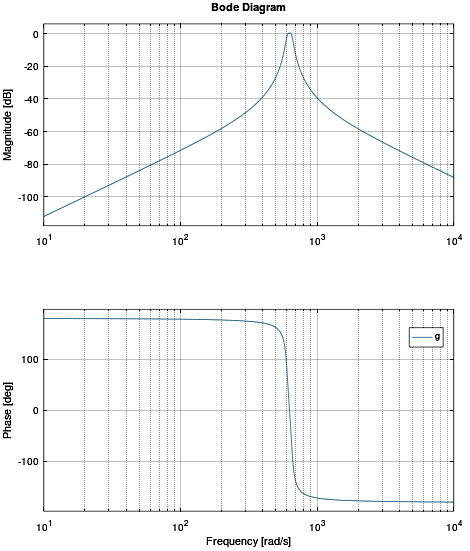
\includegraphics[scale=0.7]{DiagramasBode.png}
\caption{Diagramas de Bode}
\end{figure}

\newpage
En primer lugar tenemos el diagrama de módulo de Bode, es decir, el módulo de 
$H(jw)$ medido en dB (decibeles) el cual viene dado por la\\ fórmula
\[20 \cdot \log(|H(jw)|) dB\]
Dado que el filtro es un pasabanda era lo esperable
observar que para frecuencias bajas ($w\longrightarrow0$) y altas ($w\longrightarrow\infty$) el gráfico tendiera a $-\infty$ dado que este tipo de
filtro se caracteriza por anular la función de transferencia para dichas frecuencias.
Esto puede verse matemáticamente en base al análisis previo realizado donde se calculó que $H(0) = 0$ y $\lim_{s \to \infty} H(s) = 0$, luego 
$\lim_{x \to 0} \log(x) = -\infty$ lo cual explica lo observado en el primer gráfico.
Por último, para las frecuencias en el intervalo $(W_{0_{1}}, W_{0_{2}})$ se aprecia una ganancia que tiende a $0dB$ lo que implica una salida de igual amplitud a la de
la señal de entrada (esta es la banda que nuestro filtro deja pasar sin amortiguar).

\bigskip
El segundo gráfico es el diagrama de fase de Bode (en grados sexagesimales). 
Los valores de este gráfico vienen dados por la fórmula 
\[\arctan(\frac{\Im(H(jw))}{\Re(H(jw)})\]
Dado que el numerador de la función se compone de un único término $3948 \cdot s^2$ 
tenemos que la constante positiva aporta $0\degree$ mientras que el $s^2$ aporta
$180\degree$ (recordemos que $s=jw$ lo cual tiene un ángulo de $90\degree$, luego elevar al cuadrado duplica el ángulo y obtenemos $180\degree$).

\bigskip
Al acercarnos a las frecuencias $W_{0}$ de los polos vemos como empieza a disminuir el ángulo a un ritmo de $-180 \frac{grad}{dec}$ aproximadamente. En rigor, en principio hay un intervalo donde disminuye $-90 \frac{grad}{dec}$ pero dicho intervalo no es apreciable dada la escala y cercanía entre los $W_{0}$. 
Finalmente, una vez alcanzado el valor $W=10 \cdot W_{0}$ los polos ya no aportan
pendiente decreciente y se estabiliza el gráfico nuevamente, quedando en este caso
en $-180\degree$ aproximadamente.

\newpage
\section*{Respuesta gráfica del sistema a distintas señales}

A continuación se presentan gráficos de respuestas del sistema a distintos tipos
de señales y frecuencias.

\subsubsection*{Respuesta al escalón}

\begin{figure}[h!]
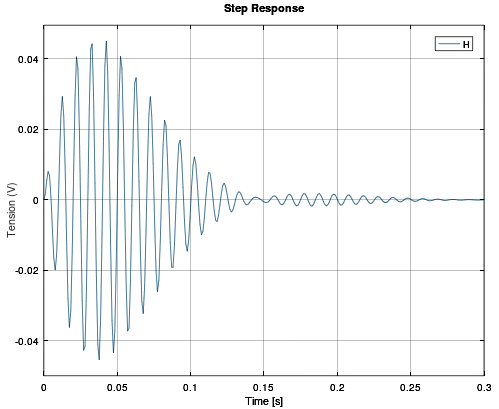
\includegraphics[scale=0.7]{RtaEscalon.png}
\caption{Respuesta al escalón}
\end{figure}

Vemos que al ser un filtro pasabanda nuestro sistema no reacciona al instante 
$t=0^{+}$ el cual correspondería a una frecuencia $w\longrightarrow \infty$.
Luego obtenemos una respuesta oscilatoria (esperable dado que se tienen polos
complejos) que va tendiendo a cero a medida que pasa el tiempo (debido a los factores
exponenciales decrecientes provenientes de la parte real negativa de las raíces de los polos). Cuando $t\longrightarrow \infty$ tenemos que $w\longrightarrow 0$ y
se da, como era esperable dado el análisis previo, que la respuesta del sistema tiende a cero y logrando estabilizarse.

\bigskip
Si analizamos el instante donde $t = 0,15s$ podemos observar un comportamiento en principio extraño, donde nuestra señal disminuye considerablemente para luego volver a crecer y finalmente anularse. Esto se debe a que la respuesta al escalón es una función compuesta por funciones senoidales de igual fase y frecuencias muy cercanas entre sí (recordemos que $W_{0_{1}} \approx 607,3\frac{r}{s}$ y $W_{0_{2}} \approx 650,2\frac{r}{s}$) donde la amplitud de estas senoidales viene dada por funciónes exponenciales negativas de $\tau$ (\textit{taus}) cercanos entre sí ($\tau_{1} \approx 21,03s$, $\tau_{2} \approx 23,03s$), lo que da como resultado el efecto de \textit{batido} para esa intervalo de tiempo específico. Los siguientes gráficos ayudan a ejemplificar este efecto de batido. \footnote{https://ricuti.com.ar/no\_ me\_ salen/ondas/Ap\_ ond\_ 14.html}

\bigskip
\begin{figure}[h!]
\centering
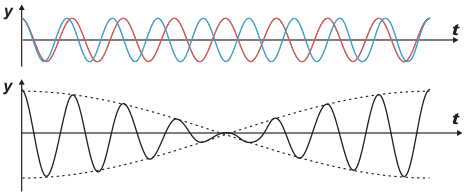
\includegraphics[scale=1]{EfectoBatido.png}
\caption{Efecto de batido entre dos funciones senoidales}
\end{figure}

Si no tuvieramos las exponenciales negativas que nos "matan" la señal observaríamos lo siguiente a medida que avanzacemos en la escala del tiempo.

\bigskip
\begin{figure}[h!]
\centering
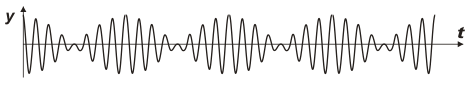
\includegraphics[scale=1]{EfectoBatidoExtendido.png}
\caption{Efecto de batido extendido en el tiempo}
\end{figure}

\newpage
\subsubsection*{Respuesta al impulso}

\begin{figure}[h!]
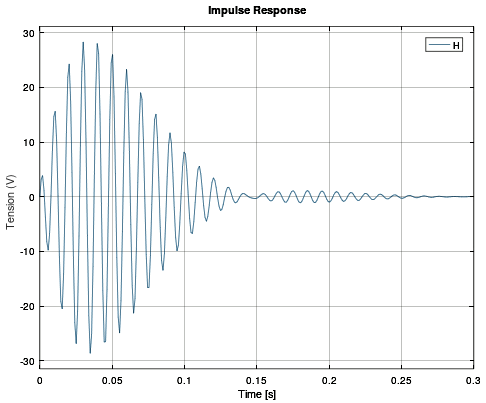
\includegraphics[scale=0.7]{RtaImpulso.png}
\caption{Respuesta al impulso}
\end{figure}

La respuesta al impulso es matemáticamente la derivada de la respuesta al escalón,
lo que dará como resultado que en los valores de $t$ donde la respuesta al escalón
alcance un máximo o mínimo entonces en la respuesta al impulso obtendremos un cero.
Puede observarse sencillamente esto en el $t$ alineado con la barra horizontal 
del valor $0 V$, donde para la respuesta al escalón se ve que se alcanza un máximo
mientras que la respuesta al impulso vale cero. Vemos que en esta respuesta también
tenemos el efecto de batido para $t = 0,15s$ lo cual es esperable dado que la derivada de la respuesta al escalón (la respuesta al impulso que estamos graficando) esta compuesta por términos similares.


\newpage
\subsubsection*{Respuesta a senoidales}

\begin{figure}[h!]
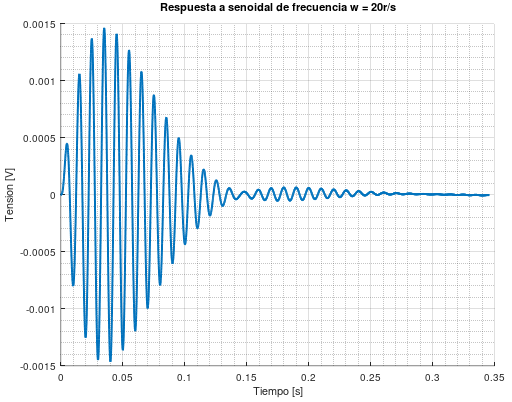
\includegraphics[scale=0.96]{RtaSenoidalBajo.png}
\caption{Respuesta a la senoidal de frecuencia $w = 20\frac{r}{s}$}
\end{figure}

Para una señal senoidal de frecuencia $w = 20\frac{r}{s}$ y $1V$ de amplitud vemos que se repite la forma de la respuesta al escalón para la las primeras décimas de segundo (componente transitoria) para finalmente tender a cero en el estado permanente, coincidiendo con el comportamiento esperado del filtro dado que es un pasabanda y por lo tanto tenderá a anular las señales de baja frecuencia.

\newpage
\begin{figure}[h!]
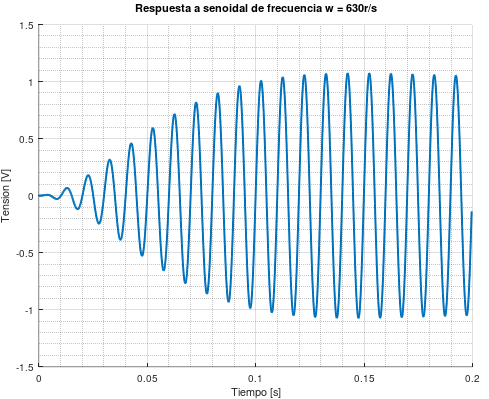
\includegraphics[scale=1]{RtaSenoidalMedio.png}
\caption{Respuesta a la senoidal de frecuencia $w = 630\frac{r}{s}$}
\end{figure}

Vemos que para una señal senoidal de frecuencia $w = 630\frac{r}{s}$ y amplitud
$1V$ al estabilizarse la respuesta obtenemos que la amplitud de la misma coincide aproximadamente con la de la señal senoidal. Esto coincide con el análisis
previo de la función de transferencia, ya que $w = 630\frac{r}{s}$ se encuentra a mitad de camino entre los $W_{0}$ calculados ($W_{0_{1}} \approx 607,3 \frac{r}{s}$ y 
$W_{0_{2}} \approx 650,2 \frac{r}{s}$) y vimos en el diagrama de Bode que para la banda de frecuencias con $W_{0_{i}}$ de extremos la ganancia era de aproximadamente $0dB$, lo que significa que la la salida mantiene la amplitud de la entrada, tal y como podemos apreciar para la respuesta a esta señal senoidal.

\newpage
\begin{figure}[h!]
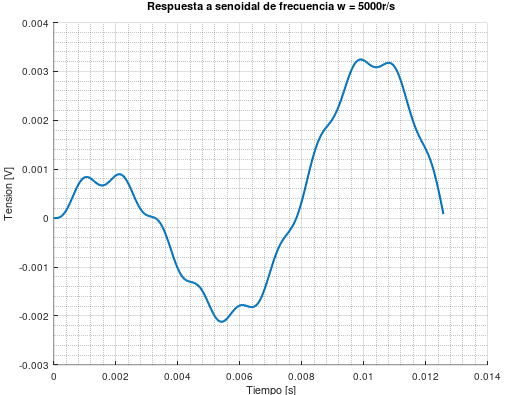
\includegraphics[scale=0.98]{RtaSenoidalAlto.png}
\caption{Respuesta a la senoidal de frecuencia $w = 5000\frac{r}{s}$}
\end{figure}

Por último tenemos que para una señal senoidal de frecuencia $w = 5000\frac{r}{s}$ y amplitud $1V$ se presenta una respuesta similar a la de baja frecuencia, donde la respuesta de nuestro sistema se ve muy atenuada(como vimos previamente para la señal senoidal de frecuencia $w = 20\frac{r}{s}$). Vemos que inicialmente presenta una respuesta parecida a la del escalón para su estado transitorio, y una vez alcanzado el estado
estacionario la respuesta es de forma senoidal con amplitud tendiendo a cero (como es esperable, mientras más aumentemos la frecuencia dicha amplitud tenderá más aún a cero). La atenuación de la señal senoidal coindice con el hecho de que nuestro filtro es un pasabanda y por lo tanto anulará las señales de altas frecuencias.

\newpage
\subsubsection*{Respuesta a la cuadrada}

Esta sección se dividirá en dos subsecciones, en la primera analizaremos las cuadradas de frecuencias relacionadas con la de $W_{0_{1}} \approx 607,3 \frac{r}{s}$ y en la siguiente para las cuadradas de frecuencias relacionadas a $W_{0_{2}} \approx 607,3 \frac{r}{s}$. Recordemos que $f = \frac{W}{2 \cdot \pi}$.

\subsubsection*{Frecuencia $f_{0_{1}}$}

Para $W_{0_{1}}$ tenemos que $f_{0_{1}} = \frac{W_{0_{1}}}{2 \cdot \pi} \approx 96,65Hz$.

\begin{figure}[h!]
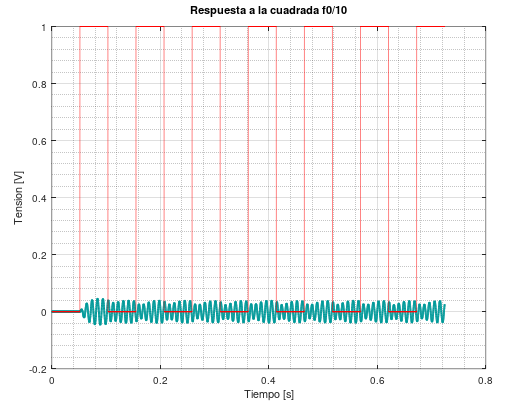
\includegraphics[scale=1]{RtaCuadradaWo11.png}
\caption{Respuesta a la cuadrada de frecuencia $\frac{f_{0_{1}}}{10}$}
\end{figure}

Para una señal cuadrada de frecuencia $\frac{f_{0_{1}}}{10} \approx 9,665Hz$ vemos que 
la respuesta oscila constantemente alrededor de cero, y dado que es un filtro pasabanda no reacciona a ninguno de los flancos (los flancos tendrían una frecuencia
prácticamente infinita y el filtro pasabanda, como vimos antes, no reacciona a dicha frecuencia). Comparando gráficos vemos que la respuesta a esta señal cuadrada se asemeja a la respuesta al escalón con la diferencia de que, debido a que estamos excitandola constantemente y no dejamos que alcance frecuencia cero, la respuesta nunca se extingue.

\bigskip
\begin{figure}[h!]
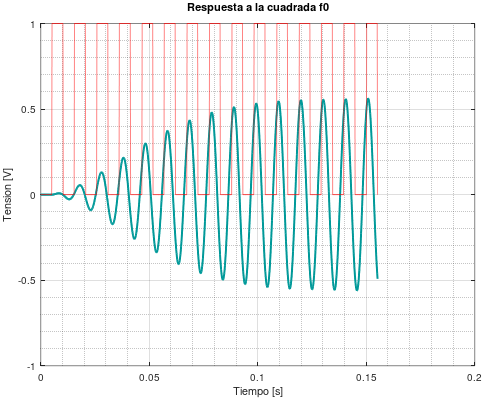
\includegraphics[scale=1]{RtaCuadradaWo12.png}
\caption{Respuesta a la cuadrada de frecuencia $f_{0_{1}}$}
\end{figure}

Para la señal cuadrada de frecuencia $f_{0_{1}} \approx 96,65Hz$ tenemos que la 
respuesta, una vez estabilizada, es una senoidal de amplitud igual a la mitad de la 
de la señal cuadrada ($0,5V$ en este caso). Esto es lógico si vemos que la señal 
cuadrada generada se puede pensar como una continua de $0,5V$ más una cuadrada centrada en cero de $0,5V$ de amplitud. Dado que la frecuencia de la cuadrada esta en el rango de frecuencias entre los $W_{0_{i}}$ (más especificamente, coincide con el extremo $W_{0_{1}}$) entonces  la señal no se ve atenuada significativamente por el filtro. Por otro lado, el tiempo que tarda en estabilizarse la señal está relacionado con el tiempo que tarda el filtro en estabilizar la respuesta a la continua.

\newpage
\begin{figure}[h!]
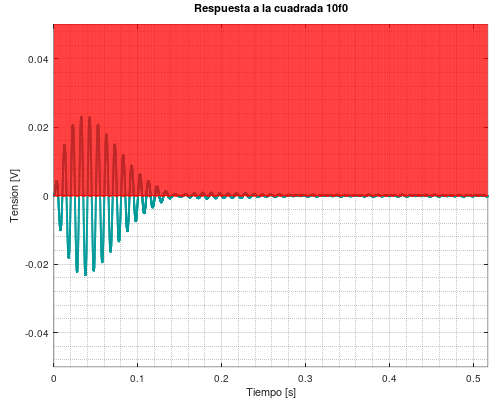
\includegraphics[scale=1]{RtaCuadradaWo13.png}
\caption{Respuesta a la cuadrada de frecuencia $f_{0_{1}} \cdot 10$}
\end{figure}
\afterpage{\clearpage}

Para la señal cuadrada de frecuencia $10 \cdot f_{0_{1}} \approx 966,5Hz$ tenemos que una vez alcanzado el estado permanente la respuesta oscila alrededor de los $0V$ cercanamente, coincidiendo con el comportamiento esperado del pasabanda para frecuencias mayores a las de la banda que deja pasar el filtro (que recordemos que va de $f_{0_{1}}$ a $f_{0_{2}}$, y debido a que estas frecuencias son cercanas entre sí entonces diez veces la primera ya se aleja considerablemente de dicha banda). El estado transitorio presenta la forma de la respuesta al escalón debido a la tensión continua que tiene la señal cuadrada. Lo que aparenta ser un rectángulo rojo en realidad son varios pulsos de la cuadrada pero debido a su alta frecuencia estos pulsos son muy cercanos entre sí (nuevamente, la señal cuadrada tiene amplitud 1V).

\subsubsection*{Frecuencia $f_{0_{2}}$}

Dado que $W_{0_{2}} \approx 650,2\frac{r}{s}$ para este caso tendremos que $f_{0_{2}} = \frac{W_{0_{2}}}{2 \cdot \pi} \approx 103,5Hz$. Debido a que las frecuencias $f_{0_{i}}$ son tan cercanas entre sí tendremos que los siguientes gráficos serán extremadamente parecidos a los anteriores, por lo que todo lo explicado previamente aplica de igual manera a lo siguiente y no será repetido.

\begin{figure}[h!]
\centering
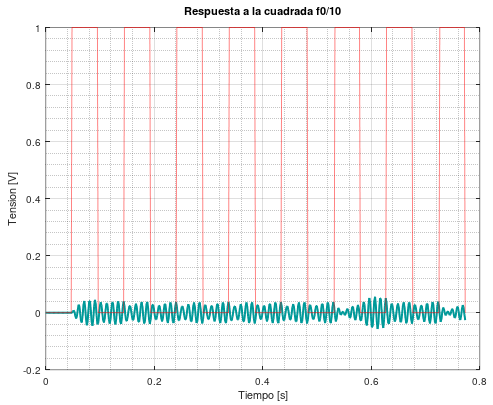
\includegraphics[scale=0.85]{RtaCuadradaWo21.png}
\caption{Respuesta a la cuadrada de frecuencia $\frac{f_{0_{2}}}{10}$}
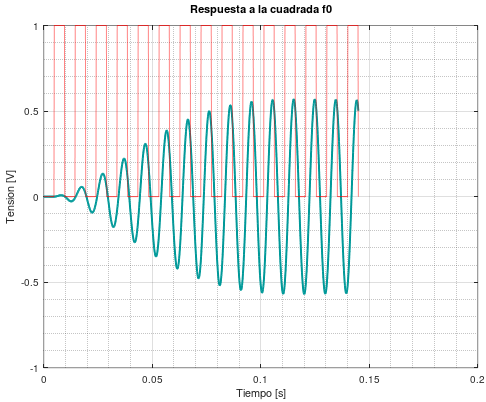
\includegraphics[scale=0.85]{RtaCuadradaWo22.png}
\caption{Respuesta a la cuadrada de frecuencia $f_{0_{2}}$}
\end{figure}
\clearpage

\begin{figure}[ht!]
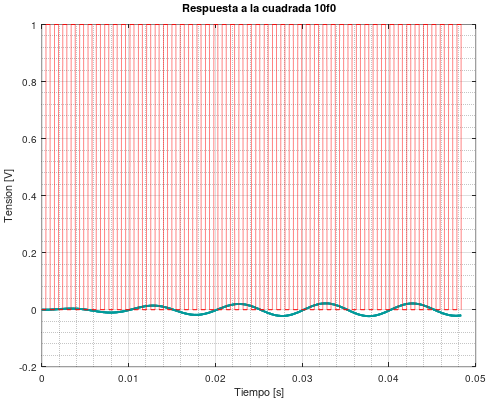
\includegraphics[scale=1]{RtaCuadradaWo23.png}
\caption{Respuesta a la cuadrada de frecuencia $f_{0_{2}} \cdot 10$}
\end{figure}


\section*{Circuito propuesto}

Se propone un circuito compuesto por dos Multiple Feedback Band-pass Filter (MFBP) . La elección del MFBP por sobre otro tipo de filtros se debe a la 
facilidad que aporta diseñar el circuito con este tipo de filtro. La principal
desventaja de este filtro es que es complicado conseguir secciones de frecuencias y Q altos ($Q > 20$) debido a las limitaciones de la ganancia de lazo abierto del amplificador operacional integrado.\footnote{https://www.analog.com/media/en/training-seminars/design-handbooks/Op-Amp-Applications/Sections5-5-to-5-8.pdf, página 5.70} Dado que nuestra transferencia se compone por valores de $Q$ bajos ($Q < 20$) no habrá problemas en utilizar este tipo de filtro.

\subsection*{Transferencia del MFPB}

A continuación se presenta un diagrama de un filtro Multiple Feedback Band-pass (MFBP).

\begin{figure}[h!]
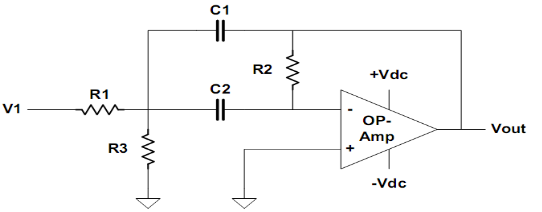
\includegraphics[scale=0.9]{MFBP.png}
\caption{Filtro MFBP}
\end{figure}

\afterpage{\clearpage}
Para este tipo de filtro se tiene una transferencia del tipo
\[H_{MFBP}(s) = -H_{0} \cdot \frac{\frac{W_{0}}{Q} \cdot s}{s^2 + \frac{W_{0}}{Q} \cdot s + W_{0}^2}\]

Para simplificar las expresiones y cuentas tomaremos $C1 = C2 = C$. Resolviendo el circuito mediante el método de nodos obtenemos que la función de transferencia puede expresarse como

\bigskip
\[H_{MFBP}(s) = -\frac{R_{2}}{2 \cdot R_{1}} \cdot \frac{\frac{2}{C \cdot R_{2}} \cdot s}{s^2 + \frac{2}{C \cdot R_{2}} \cdot s + \frac{1+\frac{R_{1}}{R_{3}}}{C^2 \cdot R_{1} \cdot R_{2}}}\]

De las anteriores dos expresiones podemos inferir que
\[H_{0} = \frac{R_{2}}{2 \cdot R_{1}}\]
\[\frac{W_{0}}{Q} = \frac{2}{C \cdot R_{2}}\]
\[W_{0}^2 = \frac{1+\frac{R_{1}}{R_{3}}}{C^2 \cdot R_{1} \cdot R_{2}}\]

Despejando las $R_{i}$ en función de las demas variables obtenemos
\[R_{2} = \frac{2 \cdot Q}{C \cdot W_{0}}\]
\[R_{1} = \frac{R_{2}}{2 \cdot H_{0}}\]
\[R_{3} = \frac{R_{1}}{\frac{2 \cdot Q^2}{H_{0}} - 1}\]

donde $Q$ y $W_{0}$ son datos provenientes de nuestra función de transferencia, por lo que es cuestión tan solo de seleccionar un C adecuado, reemplazar y obtener los $R_{i}$. Antes de proceder a calcular los valores de estos elementos debemos expresar 
la función de transferencia $H(s)$ de forma tal que podamos aplicarle las ecuaciones previas. 

\bigskip
Previamente teníamos que
\[H(s) \approx \frac{3948 \cdot s^2}{(s^2+42,81 \cdot s + 607,3^2)
\cdot (s^2+46,05 \cdot s + 650,2^2)}\]

Reescribiendolo para que se adapte a la forma de los filtros MFBP\\ tendríamos
\[H(s) \approx 2 \cdot \frac{42,81 \cdot s}{(s^2+42,81 \cdot s + 607,3^2)}
\cdot \frac{46,05 \cdot s}{(s^2+46,05 \cdot s + 650,2^2)}\]

de forma tal que tenemos dos filtros MFBP, por lo tanto tendremos que encontrar las constantes $H_{0}$, $C$, $R_{1}$, $R_{2}$ y $R_{3}$ para cada uno. 

\section*{Cálculo de los componentes}

Comenzaremos calculando los valores para el MFBP de frecuencia \\$W_{0} \approx 607,3 \frac{r}{s}$ y $Q \approx 14,19$. La idea es conseguir valores ideales de resistencias que se aproximen lo más posible a valores normalizados (de forma tal de disminuir el error al normalizar) manteniendonos en un rango de resistencias de $1K\Omega$ a $1M\Omega$.
Para esto eligiremos el valor del capacitor C (normalizado) que de mejores resultados; dicho capacitor debe tener un valor de entre $1nF$ y $1 \mu F$.

\bigskip
El otro factor a variar junto con el C es el $H_{0}$ del MFBP. Tenemos que para la transferencia $H(s)$ debe suceder que $H_{0} \approx 2$, para lo cual debemos lograr que la multiplicación entre los $H_{0}$ de los filtros MFBP den aproximadamente 2. Si bien hay infinitas combinaciones posibles en la teoría, en la práctica nos vemos limitados por las otras condiciones del sistema. 

\bigskip
Para encontrar la combinación de componentes que minimizase el error relativo de $W_{o}$ y $Q$ inicialmente se fueron proponiendo valores a los capacitores y ganancias de cada filtro. Tras un extenso análisis resultó evidente que el segundo filtro era muy difícil de aproximar las resistencias normalizadas a los valores ideales de las resistencias calculadas debido a los valores particulares de $W_{0}$ y $Q$ del mismo. Debido a esto se desarrolló un algoritmo que analizase todas las combinaciones de capacitores comerciales entre $1nF$ y $1uF$ posibles para ambos filtros, y para cada combinación variase la ganancia del primer filtro $H_{o_{1}}$ (donde la ganancia del segundo filtro se calcula mediante $H_{0_{2}} = \frac{2}{H_{0_{1}}}$) comenzando por $H_{0_{1}} = 0,01$ hasta $H_{0_{1}} < 70$ con paso $0,01$. 

\bigskip
Una vez obtenidos los valores normalizados de las resistencias calculadas el algoritmo calcula con ellas el $W_{0}$ y $Q$ y procede a calcular el error relativo de cada uno. Con los cuatro errores relativos obtenidos (porque hay dos filtros) procede a sumarlos para obtener una aproximación del error relativo total, y analiza si este es menor a la anterior mejor combinación obtenida. De esta forma se consigue la mejor combinación de resistencias normalizadas para nuestro circuito.
Es importante recalcar que no se considera el error de $H_{0}$ para el algoritmo ya que este en última instancia podría mejorarse con un filtro plano, la idea es que el algoritmo se enfoque en minimizar el error en $W_{0}$ y $Q$.

\bigskip
Los resultados obtenidos fueron interesantes. A continuación se presentan los mejores resultados posibles para tres condiciones distintas.

\clearpage
\begin{list}{•}
\item Manteniéndose entre resistencias de $1K\Omega$ y $1M\Omega$ utilizando resistencias de tolerancia $10\%$ únicamente

\vspace{10 mm}

\begin{figure}[h!]
\centering
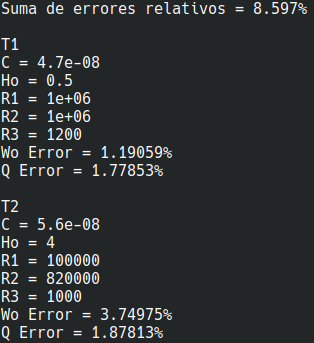
\includegraphics[scale=1]{ResultadosPrimerCaso.png}
\caption{Primera simulación}
\end{figure}

Vemos que si intentamos mantenernos en los valores recomendados por el trabajo práctico obtenemos los peores resultados con diferencia. Como se mencionó previamente
el principal culpable es el segundo filtro (T2), aportándonos mucho error relativo
para el $W_{0}$. Si simulamos el circuito en el programa \textit{LTSpice} y graficamos los diagramas de Bode se obtiene un error de aproximadamente $5,6dB$ en el diagrama de módulo. Si bien se podría disminuir este error, se requeriría de varias resistencias de menor tolerancia y presets, lo cual no es ideal. Veremos que pasa con los siguientes casos.

\newpage

\item
\item Manteniéndose entre resistencias de $100\Omega$ y $1M\Omega$ utilizando resistencias de tolerancia $10\%$ únicamente

\vspace{10 mm}

\begin{figure}[h!]
\centering
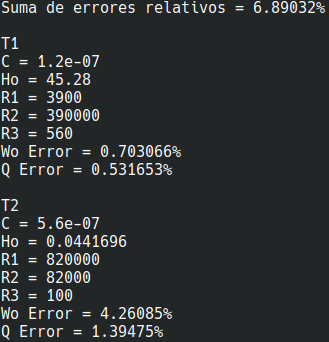
\includegraphics[scale=1]{ResultadosSegundoCaso.png}
\caption{Segunda simulación}
\end{figure}

Vemos que para este caso obtenemos una mejora leve con respecto al anterior, disminuyendo el error relativo total aproximadamente $1,7\%$. Logramos conseguir una mejor aproximación para el primer filtro sin embargo el segundo filtro aumentó su error de $W_{0}$ considerablemente. Si simulamos el circuito con estos valores en el
\textit{LTSpice} obtenemos un error aproximado de $6dB$ lo cual es más error que en nuestra anterior simulación (esto se debe a que la suma de errores relativos es tan sólo una estimación del error real, y por otro lado solo estamos analizando el error en dB y no en la banda de frecuencias). Veremos que sucede con el último análisis.

\newpage
\item Manteniéndose entre resistencias de $100\Omega$ y $1M\Omega$ utilizando resistencias de tolerancia $10\%$ pero permitiendo usar una del $5\%$

\vspace{10 mm}

\begin{figure}[h!]
\centering
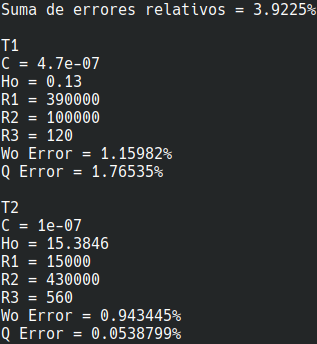
\includegraphics[scale=1]{ResultadosTercerCaso.png}
\caption{Tercera simulación}
\end{figure}

Por último le permitimos al algoritmo hacer uso de una sola resistencia de tolerancia $5\%$ y ver si conseguimos algún tipo de mejora substancial. Afortunadamente conseguimos una mejora considerable de aproximadamente el $3\%$. No sólo eso sino que logramos bajar también considerablemente el promedio de errores relativos, lo que resulta en una mejora mucho mayor a la esperada. Si simulamos el circuito en el \textit{LTSpice} 
ahora tenemos un error de aproximadamente $0,2dB$ únicamente, y logramos una aproximación de la banda de frecuencias del pasabanda muy cercana al ideal.

\end{list}

\bigskip
En base a lo expuesto se optó por la última combinación de valores. Para resumir 
se presenta la siguiente tabla con los valores de los componentes y sus respectivos errores relativos, de igual forma se presentan los valores ideales y aproximados de $W_{0}$, $Q$ y $H_{0}$.

\begin{figure}[!ht]
\centering
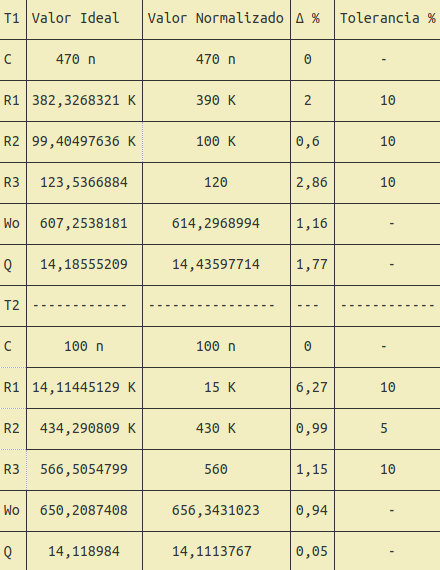
\includegraphics[scale=1]{tablaValores.png}
\caption{Valores obtenidos para el circuito}
\end{figure}

\newpage
En base a los valores de $H_{0}$, $W_{0}$ y $Q$ calculados en la tabla obtenemos una función de transferencia tal que
\[H_{n}(s) \approx \frac{(-0,128) \cdot 42,55 \cdot s}{s^2 + 42,55 \cdot s + 614,30^2} \cdot \frac{(-14,33) \cdot 46,51 \cdot s}{s^2 + 46,51 \cdot s + 656,34^2}\]

Multiplicando ambos factores obtenemos finalmente que

\[H_{n}(s) \approx \frac{3637 \cdot s^2}{(s^2 + 42,55 \cdot s + 614,30^2)
\cdot (s^2 + 46,51 \cdot s + 656,34^2)}\]

donde $H_{n}(s)$ es la función de transferencia obtenida tras normalizar los componentes.

\section*{Diagramas de $H_{n}(s)$}

A continuación se presentan los diagramas de Bode y la respuesta al escalón de $H_{n}(s)$. Se mostrarán primero los gráficos por separado para \\poder apreciarlo mejor, y luego se superpondrán con los correspondientes a $H(s)$ para tener una idea de la precisión de la misma.

\subsection*{Diagramas de Bode}

\begin{figure}[h!]
\centering
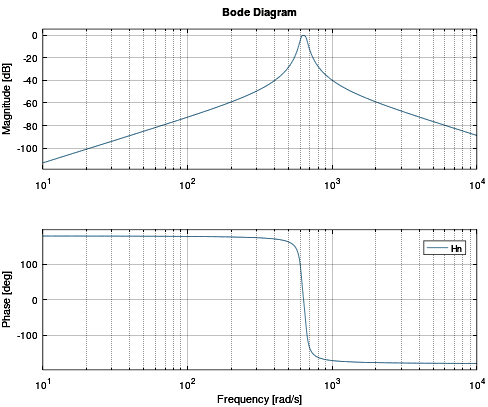
\includegraphics[scale=0.7]{DiagramasBodeN.png}
\caption{Diagramas de bode de $H_{n}(s)$}
\end{figure}
\clearpage

\begin{figure}[h!]
\centering
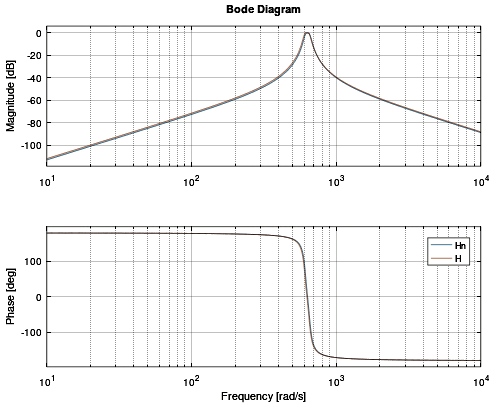
\includegraphics[scale=0.7]{DiagramasBodeComp.png}
\caption{Diagramas de bode de $H_{n}(s)$ y $H(s)$}
\end{figure}

Vemos que a gran escala ambos gráficos prácticamente se superponen. Para apreciar la diferencia podemos magnificar la banda de frecuencias donde la ganancia es aproximadamente $0dB$.

\begin{figure}[h!]
\centering
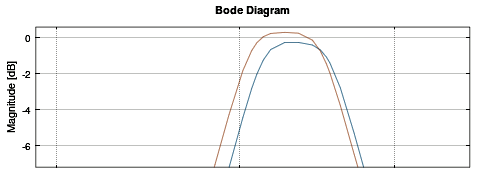
\includegraphics[scale=0.7]{DiagramasBodeCloseComp.png}
\caption{Diagramas de bode de $H_{n}(s)$ (azul) y $H(s)$ (naranja)}
\end{figure}

Vemos que el error es aproximadamente $0,5dB$. También podemos observar un ligero error en las frecuencias, esperable si consideramos que $W_{0_{1}} \approx 607,3\frac{r}{s}$ y nosotros obtuvimos un valor $W_{0_{1}} \approx 614,30\frac{r}{s}$ cuando normalizamos (lo mismo para $W_{0_{2}}$).

\subsection*{Respuesta al escalón}

\vspace{10 mm}

\begin{figure}[h!]
\centering
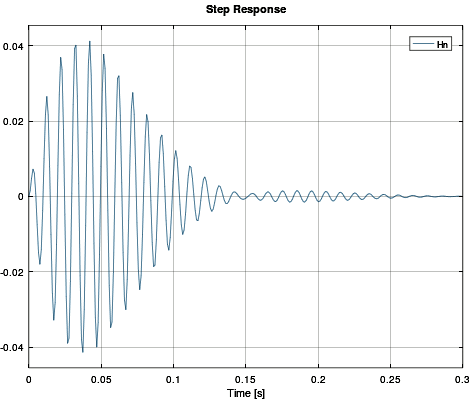
\includegraphics[scale=0.7]{RtaEscalonN.png}
\caption{Respuesta al escalón de $H_{n}(s)$}
\end{figure}
\clearpage

\begin{figure}[h!]
\centering
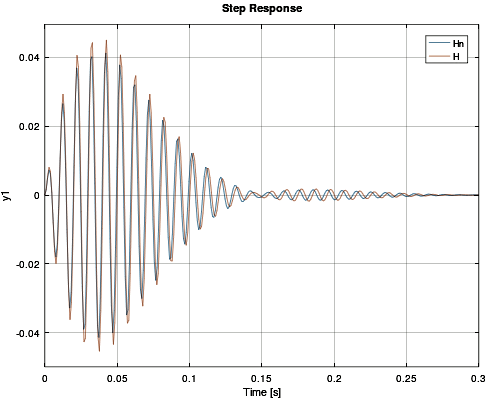
\includegraphics[scale=0.7]{RtaEscalonComp.png}
\caption{Respuesta al escalón de $H_{n}(s)$ y $H(s)$}
\end{figure}

Nuevamente ambos gráficos son muy parecidos, si bien aquí es más sencillo ver las
diferencias. A continuación se muestra un gráfico que magnifica la zona donde $t \approx 0,15s$.

\begin{figure}[h!]
\centering
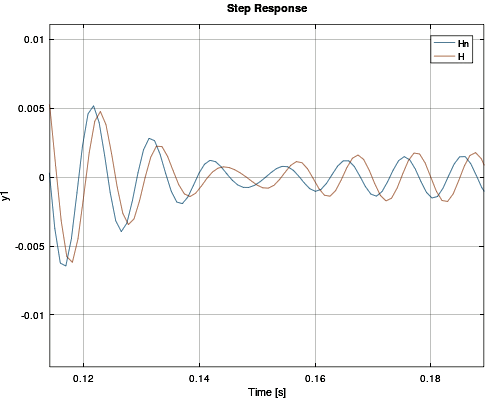
\includegraphics[scale=0.48]{RtaEscalonCloseComp.png}
\caption{Respuesta al escalón de $H_{n}(s)$ y $H(s)$}
\end{figure}

\section*{Simulación con \textit{LTSpice}}

Habiendo normalizado los valores de los componentes del circuito para conseguir la
transferencia asignada procederemos a simular el mismo mediante el programa \textit{LTSpice}. Para esto se mostrarán primero los diagramas obtenidos para las
distintas simulaciones individualmente y luego comparando con los diagramas de la
transferencia original. Finalmente se compararan todos los diagramas juntos (la función $H(s)$, la función $H_{n}(s)$ y los generados por \textit{LTSpice}).

\bigskip
Antes de proceder a mostrar los gráficos obtenidos, se presenta un esquema del circuito utilizado en el \textit{LTSpice}.

\vspace{20 mm}

\begin{figure}[h!]
\centering
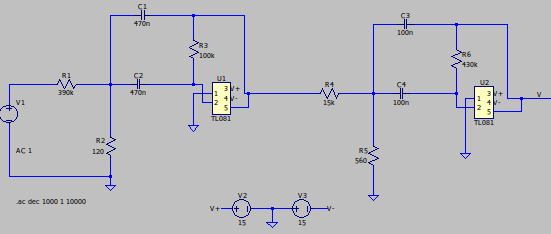
\includegraphics[scale=1]{Circuito.png}
\caption{Circuito propuesto para la transferencia asignada}
\end{figure}

\newpage
\subsection*{Diagramas de Bode}

\begin{figure}[h!]
\centering
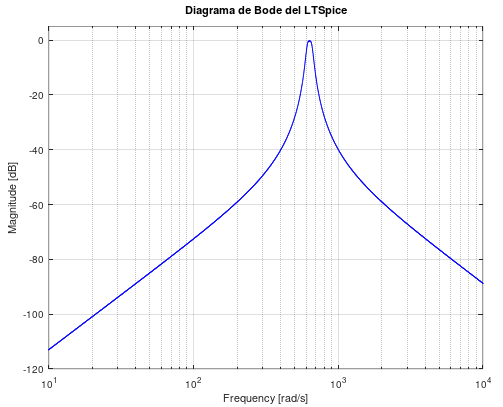
\includegraphics[scale=0.9]{MagnitudBodeSpice.png}
\caption{Diagrama de magnitud de Bode del circuito simulado en \textit{LTSpice}}
\vspace{2 mm}
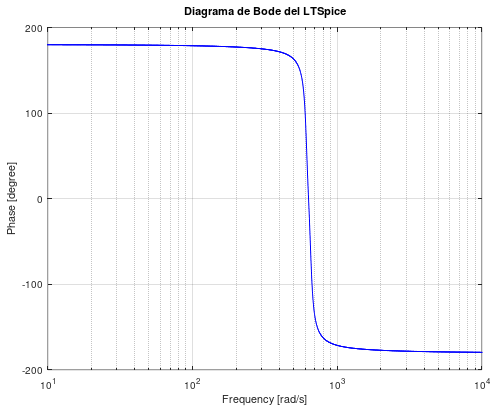
\includegraphics[scale=0.85]{PhaseBodeSpice.png}
\caption{Diagrama de fase de Bode del circuito simulado en \textit{LTSpice}}
\end{figure}

\begin{figure}[h!]
\centering
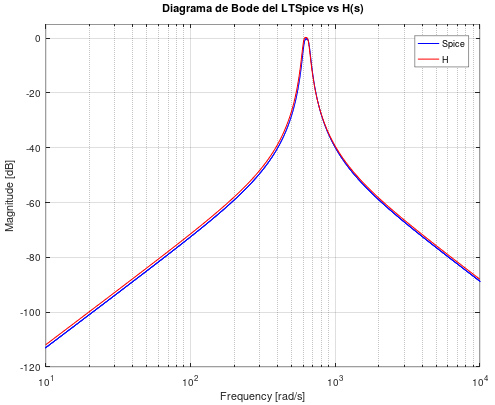
\includegraphics[scale=0.9]{MagnitudBodeSpiceComp.png}
\caption{Comparación entre H(s) y \textit{LTSpice} de la magnitud}
\vspace{2 mm}
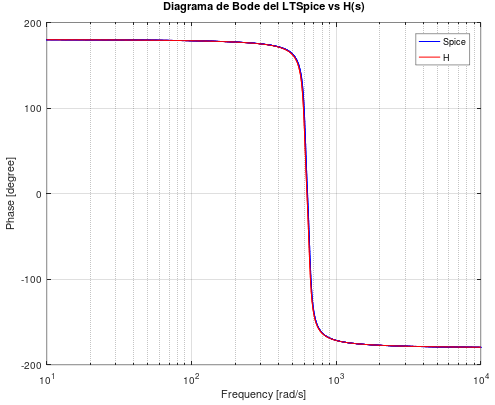
\includegraphics[scale=0.85]{PhaseBodeSpiceComp.png}
\caption{Comparación entre H(s) y \textit{LTSpice} de la fase}
\end{figure}

\subsection*{Respuesta al escalón}

\begin{figure}[h!]
\centering
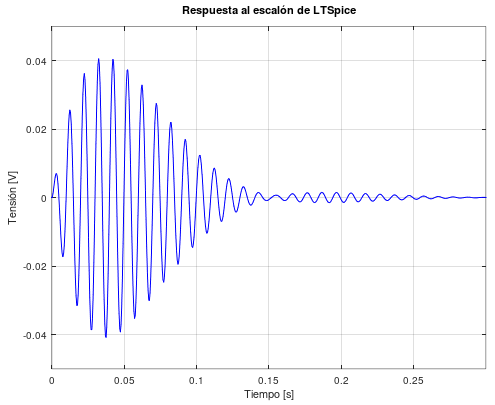
\includegraphics[scale=0.9]{rtaEscalonSpice.png}
\caption{Respuesta al escalón de \textit{LTSpice}}
\vspace{2 mm}
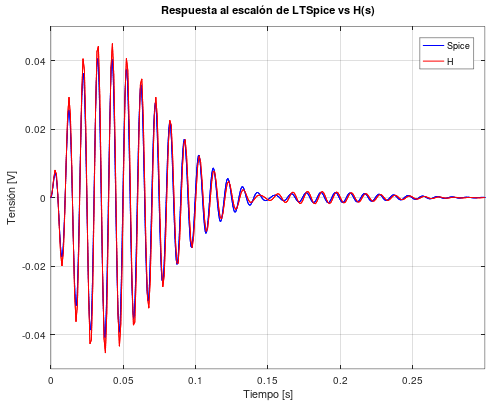
\includegraphics[scale=0.85]{rtaEscalonSpiceComp.png}
\caption{Comparación de la respuesta al escalón entre \textit{LTSpice} y H(s)}
\end{figure}

\subsection*{Respuesta a senoidales}

Las frecuencias $W_{0}$ utilizadas para las señales senoidales serán las mismas que para el el inciso \textbf{Respuesta a senoidales} de la sección \textbf{Respuesta gráfica del sistema a distintas señales}.

\begin{figure}[h!]
\centering
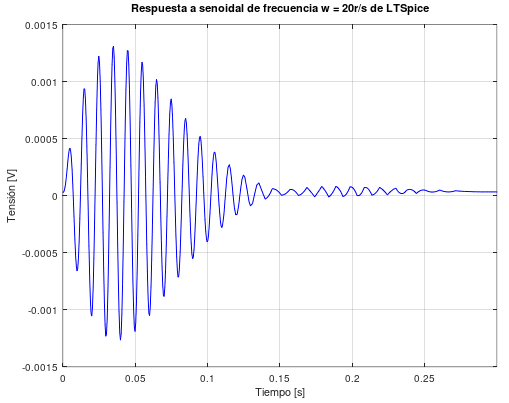
\includegraphics[scale=0.8]{rtaSenoidalBajoSpice.png}
\caption{Respuesta a señal senoidal de $w = 20 \frac{r}{s}$ de \textit{LTSpice}}
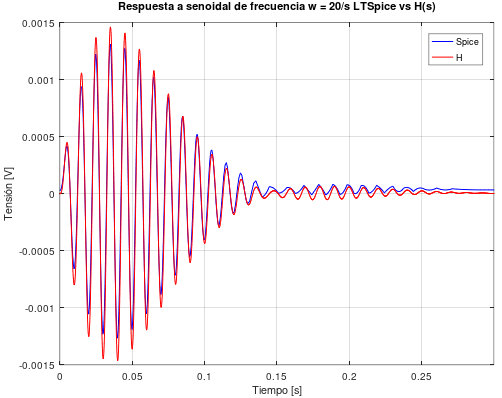
\includegraphics[scale=0.8]{rtaSenoidalBajoSpiceComp.png}
\caption{Comparación de la respuesta para H(s) vs \textit{LTSpice}}
\end{figure}
\newpage 

\begin{figure}[h!]
\centering
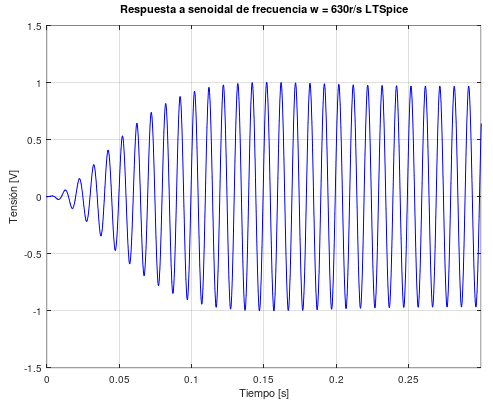
\includegraphics[scale=1]{rtaSenoidalMedioSpice.png}
\caption{Comparación de la respuesta para H(s) vs \textit{LTSpice}}
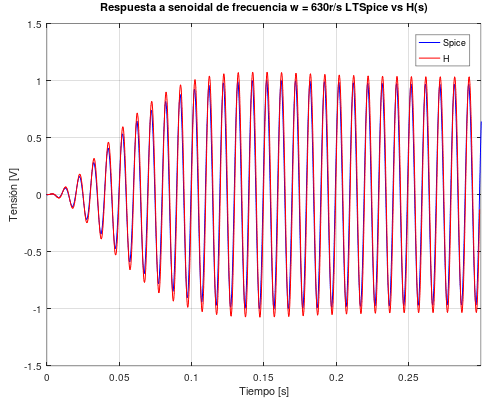
\includegraphics[scale=0.96]{rtaSenoidalMedioSpiceComp.png}
\caption{Comparación de la respuesta para H(s) vs \textit{LTSpice}}
\end{figure}

\newpage

\begin{figure}[h!]
\centering
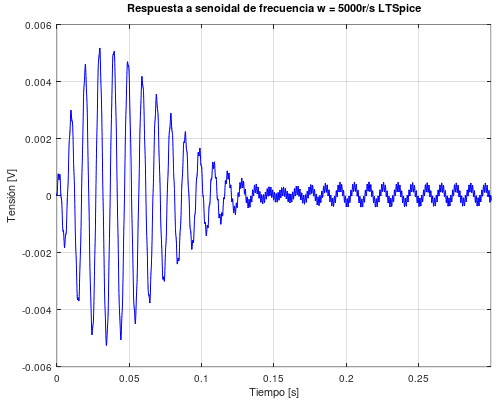
\includegraphics[scale=1]{rtaSenoidalAltoSpice.png}
\caption{Respuesta a señal senoidal de $w = 5000 \frac{r}{s}$ de \textit{LTSpice}}
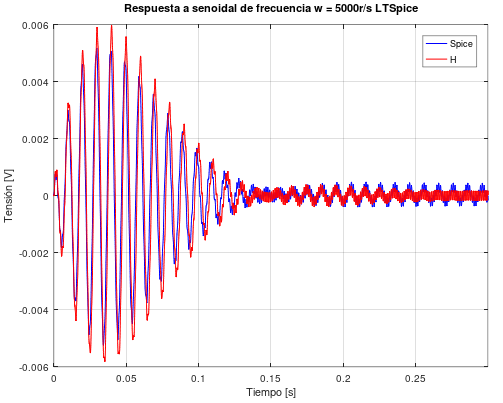
\includegraphics[scale=0.96]{rtaSenoidalAltoSpiceComp.png}
\caption{Comparación de la respuesta para H(s) vs \textit{LTSpice}}
\end{figure}
\clearpage

El siguiente gráfico magnifica la respuesta a la señal senoidal de frecuencia $w = 5000 \frac{r}{s}$ en el estado permanente para poder apreciar mejor la diferencia entre la respuesta de $H(s)$ y la respuesta del circuito normalizado generada por \textit{LTSpice}.

\begin{figure}[h!]
\centering
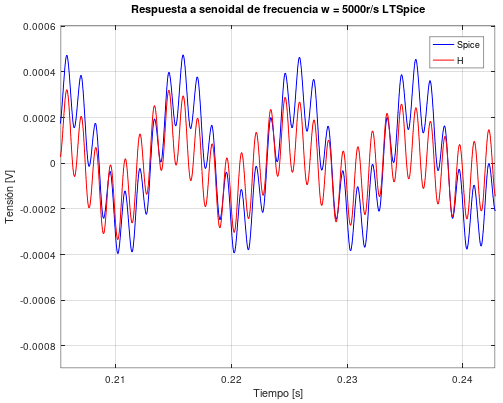
\includegraphics[scale=0.96]{rtaSenoidalAltoSpiceCloseComp.png}<
\caption{Comparación de la respuesta para H(s) vs \textit{LTSpice} magnificada}
\end{figure}

Vemos que hay una diferencia de amplitud y un desfase, esperable considerando la normalización de los componentes. Hay que considerar también que a medida que vamos avanzando hacia frecuencias altas o bajas nuestra respuesta tiende más a cero y las simulaciones son más propensas a tener errores de aproximación (como vimos para el caso de frecuencias bajas en \textit{Octave}).

\subsection*{Respuesta a la cuadrada}

Al igual que como hicimos para el ítem \textbf{Respuesta a la cuadrada} de la sección \textbf{Respuesta gráfica del sistema a distintas señales}, esta sección se dividirá en dos subsecciones, en la primera analizaremos las cuadradas de frecuencias relacionadas con la de $W_{0_{1}} \approx 607,3 \frac{r}{s}$ y en la siguiente para las cuadradas de frecuencias relacionadas a $W_{0_{2}} \approx 650,2 \frac{r}{s}$. Recordemos que $f = \frac{W}{2 \cdot \pi}$.

\subsubsection*{Frecuencia $f_{0_{1}}$}

\begin{figure}[h!]
\centering
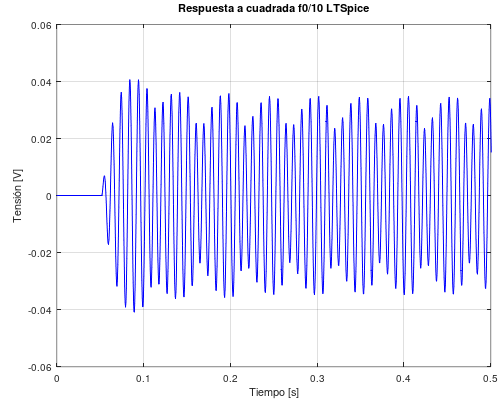
\includegraphics[scale=0.8]{rtaCuadradaBaja1Spice.png}
\caption{Respuesta a la cuadrada de frecuencia $\frac{f_{0_{1}}}{10}$ de \textit{LTSpice}}
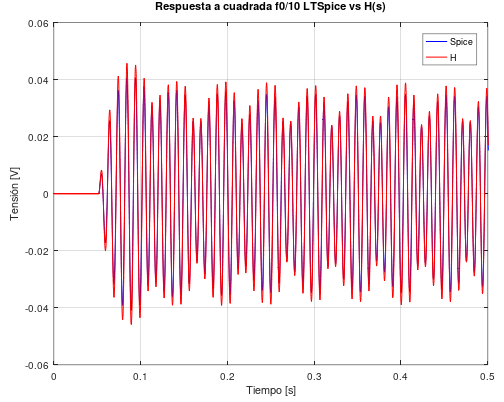
\includegraphics[scale=0.8]{rtaCuadradaBaja1SpiceComp.png}
\caption{Comparación de la respuesta para H(s) vs \textit{LTSpice}}
\end{figure}
\newpage 

\begin{figure}[h!]
\centering
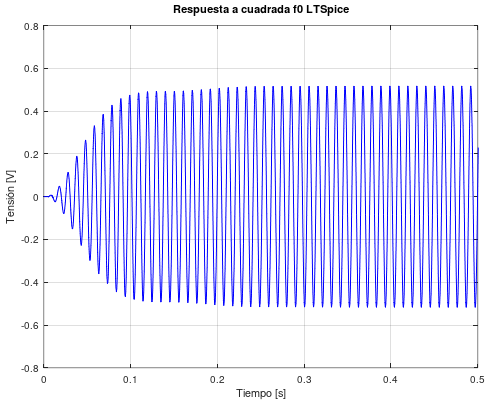
\includegraphics[scale=0.8]{rtaCuadradaMedio1Spice.png}
\caption{Respuesta a la cuadrada de frecuencia $f_{0_{1}}$ de \textit{LTSpice}}
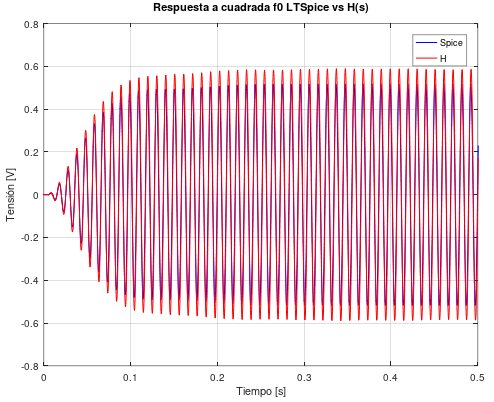
\includegraphics[scale=0.8]{rtaCuadradaMedio1SpiceComp.png}
\caption{Comparación de la respuesta para H(s) vs \textit{LTSpice}}
\end{figure}

Para la respuesta a la cuadrada de frecuencia $f_{0} = f_{0_{1}}$ tenemos un error de tensión aproximado de $0,05V$, donde la tensión del circuito normalizado simulado por \textit{LTSpice} es menor a la de $H(s)$. Esto es prevesible ya que la frecuencia angular ideal es $W_{0_{1}} \approx 607,3\frac{r}{s}$ mientras que la normalizada (que es la que simula \textit{LTSpice}) es $W_{0} \approx 614,3\frac{r}{s}$ por lo tanto tendremos menos ganancia para el normalizado y consecuentemente menos tensión, que es lo observado.

\begin{figure}[h!]
\centering
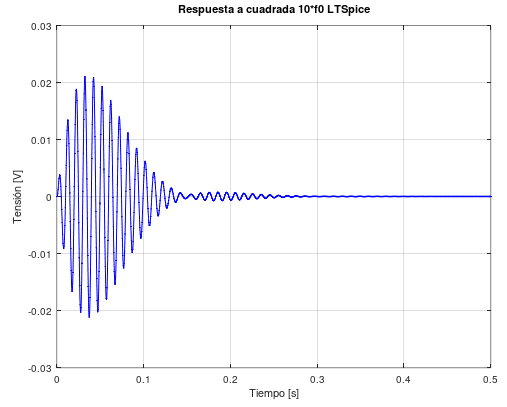
\includegraphics[scale=0.85]{rtaCuadradaAlto1Spice.png}
\caption{Respuesta a la cuadrada de frecuencia $10 \cdot f_{0_{1}}$ de \textit{LTSpice}}
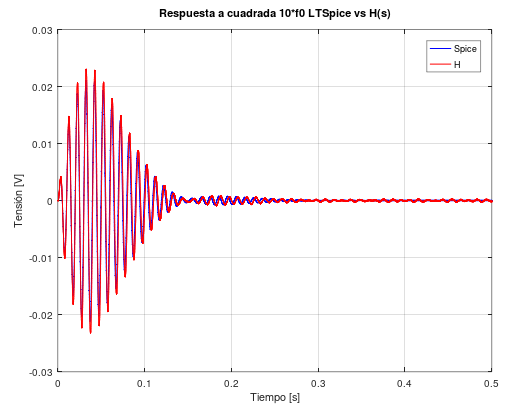
\includegraphics[scale=0.8]{rtaCuadradaAlto1SpiceComp.png}
\caption{Comparación de la respuesta para H(s) vs \textit{LTSpice}}
\end{figure}
\newpage

\subsubsection*{Frecuencia $f_{0_{2}}$}

\begin{figure}[h!]
\centering
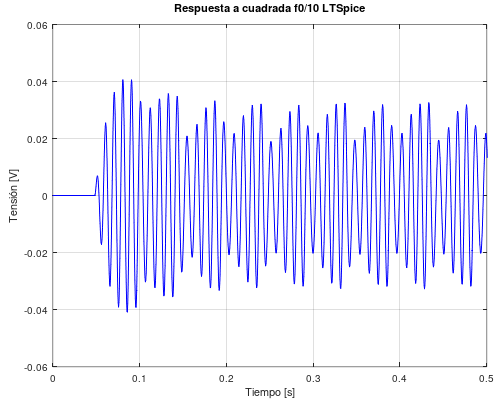
\includegraphics[scale=0.9]{rtaCuadradaBaja2Spice.png}
\caption{Respuesta a la cuadrada de frecuencia $\frac{f_{0_{2}}}{10}$ de \textit{LTSpice}}
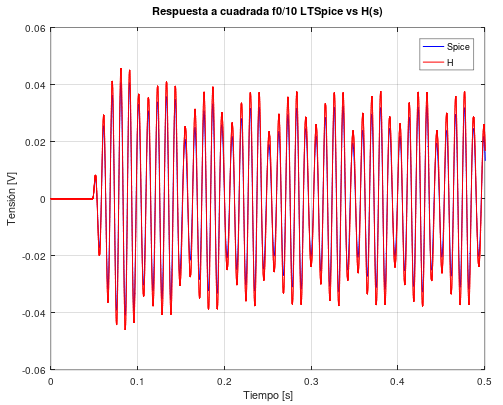
\includegraphics[scale=0.85]{rtaCuadradaBaja2SpiceComp.png}
\caption{Comparación de la respuesta para H(s) vs \textit{LTSpice}}
\end{figure}
\newpage 

\begin{figure}[h!]
\centering
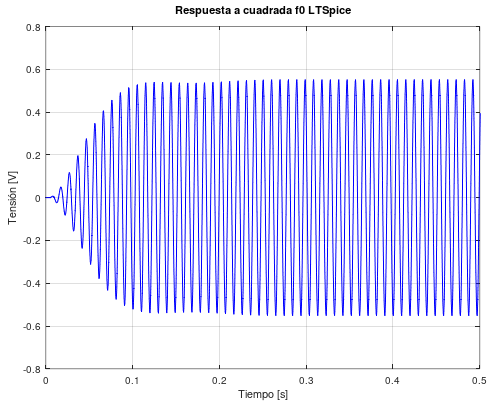
\includegraphics[scale=1]{rtaCuadradaMedio2Spice.png}
\caption{Respuesta a la cuadrada de frecuencia $f_{0_{2}}$ de \textit{LTSpice}}
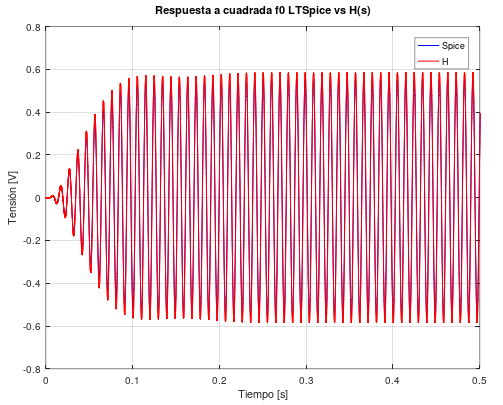
\includegraphics[scale=0.95]{rtaCuadradaMedio2SpiceComp.png}
\caption{Comparación de la respuesta para H(s) vs \textit{LTSpice}}
\end{figure}
\clearpage

\begin{figure}[h!]
\centering
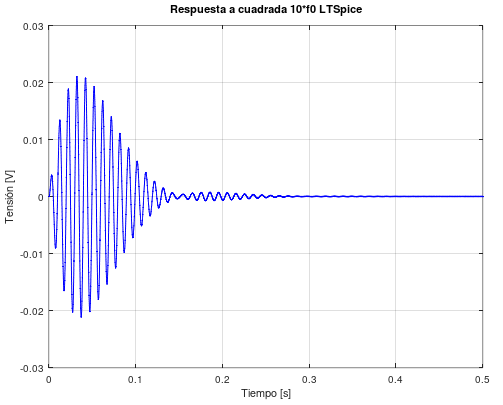
\includegraphics[scale=1]{rtaCuadradaAlto2Spice.png}
\caption{Respuesta a la cuadrada de frecuencia $10 \cdot f_{0_{2}}$ de \textit{LTSpice}}
\includegraphics[scale=0.95]{rtaCuadradaAlto2SpiceComp.png}
\caption{Comparación de la respuesta para H(s) vs \textit{LTSpice}}
\end{figure}
\clearpage

Los gráficos obtenidos para esta frecuencia son, como era esperable, iguales a los obtenidos para la frecuencia $f_{0_{1}}$ ya que ambas frecuencias son muy cercanas entre sí (esto lo habíamos aclarado ya en secciones previas) por lo tanto no hay nada remarcable para destacar.

\end{document}